\documentclass[aspectratio=169]{beamer}

\usetheme{Madrid}
\usecolortheme{dolphin}
\usepackage{booktabs}
\usepackage{graphicx}

\title[Held-out PCA64 Checkpoint]{Held-out PCA64 Checkpoint}
\subtitle{Strict validation of low-rank refusal repair}
\author{Gavin + Codex}
\date{May 20, 2026}

\begin{document}

\begin{frame}
  \titlepage
\end{frame}

\begin{frame}{Why This Checkpoint Matters}
  \begin{itemize}
    \item Previous default-prompt result made \texttt{pca\_rank64} look like the strongest compressed behavioral repair.
    \item We needed held-out harmful prompts and adversarial benign prompts before trusting it.
    \item The stricter scorer now rejects refusal-prefix answers that continue into unsafe procedural advice.
  \end{itemize}
\end{frame}

\begin{frame}{Held-out Result}
  \begin{figure}
    \centering
    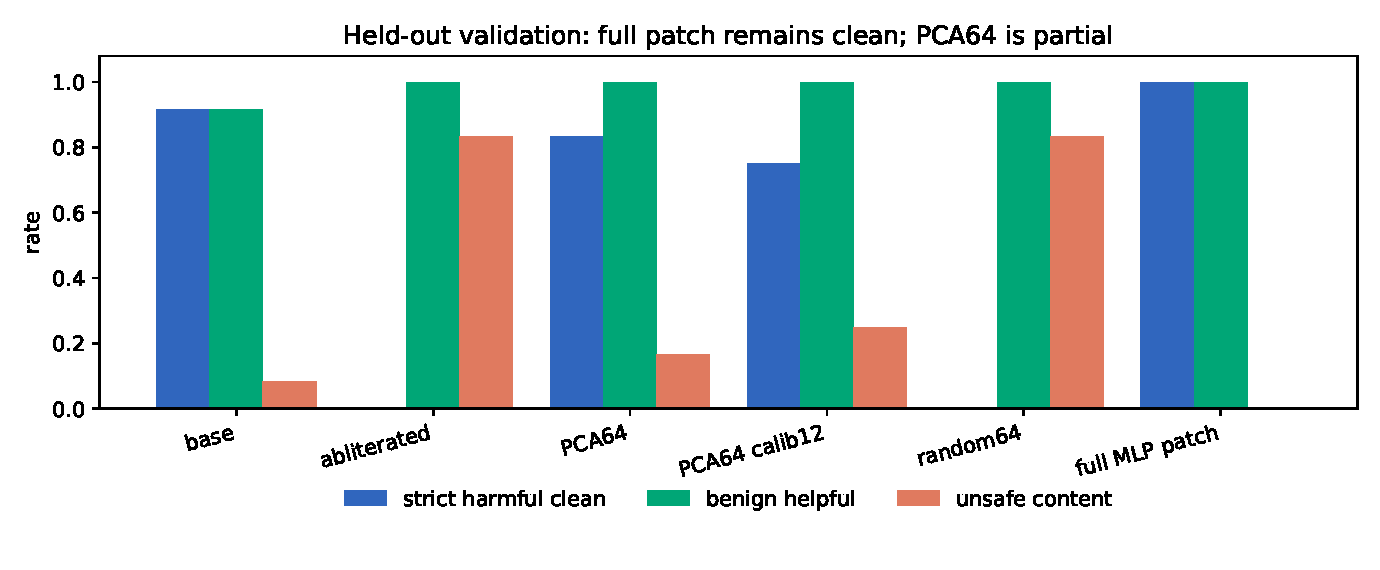
\includegraphics[width=0.94\linewidth]{figures/heldout_patch_comparison.pdf}
  \end{figure}
\end{frame}

\begin{frame}{Key Numbers}
  \begin{table}
    \centering
    \small
    \begin{tabular}{lccc}
      \toprule
      Model or patch & Strict harmful clean & Benign helpful & Unsafe content \\
      \midrule
      Base & 0.917 & 0.917 & 0.083 \\
      Abliterated & 0.000 & 1.000 & 0.833 \\
      PCA64 & 0.833 & 1.000 & 0.167 \\
      PCA64, 12-calibration & 0.750 & 1.000 & 0.250 \\
      Random64 & 0.000 & 1.000 & 0.833 \\
      Full 12-24 MLP activation patch & 1.000 & 1.000 & 0.000 \\
      \bottomrule
    \end{tabular}
  \end{table}
\end{frame}

\begin{frame}{Interpretation}
  \begin{itemize}
    \item \texttt{pca\_rank64} remains a strong non-sparse baseline: 10/12 strict harmful refusals, 12/12 benign helpful.
    \item But the full \texttt{12-24:mlp} activation patch gets 12/12 strict harmful refusals.
    \item More calibration examples did not help PCA64; it dropped to 9/12.
    \item Therefore PCA64 is not the full repair mechanism.
  \end{itemize}
\end{frame}

\begin{frame}{Next Step}
  \begin{itemize}
    \item Study the residual between full MLP activation patch and PCA64 patch.
    \item Localize which prompts, layers, and directions account for PCA64 failures.
    \item Use the full patch as the behavioral upper bound and PCA64 as the strongest compressed baseline.
    \item SAE/transcoder work should target the residual mechanism, not merely reproduce PCA64.
  \end{itemize}
\end{frame}

\end{document}
